\documentclass[pdflatex,compress]{beamer}

%\usetheme[dark,framenumber,totalframenumber]{ElektroITK}
\usetheme[darktitle,framenumber,totalframenumber]{ElektroITK}

\usepackage{soul}
\usepackage{multicol}
\usepackage{graphicx}

\title{PENGOLAHAN SINYAL DIGITAL}
\subtitle{Sinyal dan Sistem Waktu Diskrit}

\author{Tim Dosen Pengampu}

\begin{document}

\maketitle

\section{Pendahuluan}

\begin{frame}
	\frametitle{Pengantar}
	\begin{itemize}
		\item Sinyal dan sistem waktu diskrit memiliki beberapa kesamaan dengan sinyal dan sistem waktu kontinyu.
		\item Beberapa kasus yang ada di sinyal dan sistem waktu kontinyu memiliki beberapa kesamaan dengan sinyal dan sistem waktu diskrit, yang mana akan kita pelajari sepanjang perkuliahan ini.
		\item Namun, juga ada beberapa perbedaan antara sinyal dan sistem waktu diskrit dengan sinyal dan sistem waktu kontnyu.
		\item Perbedaan-perbedaan ini sangat penting dan perlu kita pahami dengan baik.
	\end{itemize}
\end{frame}

\begin{frame}
	\frametitle{Pengantar}
	\begin{itemize}
		\item Dalam domain waktu diskrit, sinyal yang diproses adalah berupa sequences $\rightarrow$ sinyal merupakan fungsi dari variabel bilangan bulat/ \textbf{integer} ($ n $).
		\item Pada slide selanjutnya, diilustrasikan contoh dari \textbf{general sequence} $ x(n) $, sebuah fungsi energi dari variabel $ n $, dan nilai dari sequence-nya dinyatakan dalam bar dengan tinggi sesuai dengan nilai sequence-nya.
		\item Perlu diperhatikan bahwa variabel $ n $ \textbf{harus berupa integer}. Jika bukan integer, maka $ x(n) $ tidak terdefinisikan.
		\item Apapun argument dalam fungsi tersebut harus bernilai \textbf{integer}.
	\end{itemize}
\end{frame}

\begin{frame}
	\frametitle{General Sequence}
	\begin{center}
		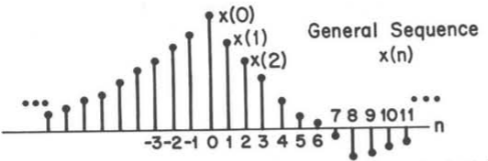
\includegraphics[width=\linewidth]{img/img001}
	\end{center}
\end{frame}

\section{Basic Signal}
\begin{frame}
	\frametitle{Unit Sample Sequence}
	\begin{itemize}
		\item Sama seperti di domain waktu kontinyu, pada domain waktu diskrit juga memiliki \textbf{basic sequence}.
		\item Basic sequence yang pertama adalah \textbf{unit sample sequence} atau \textbf{unit impulse sequence} yang diilustrasikan pada slide selanjutnya.
		\item Unit sample dinotasikan dengan $ \delta(n) $.
		\item $ \delta(n) $ bernilai 1 (\textbf{unity}) di $ n = 0 $ dan $ \delta(n) $ bernilai 0 jika $n \neq 0$ 
		\item Jika dibandingkan dengan unit sample pada domain waktu kontinyu, unit sample pada domain waktu diskrit ini memiliki definisi yang lebih pasti.
		\item Masih ingat unit sample pada domain waktu kontinyu?
	\end{itemize}
\end{frame}

\begin{frame}
	\frametitle{Unit Sample Sequence}
	\begin{center}
		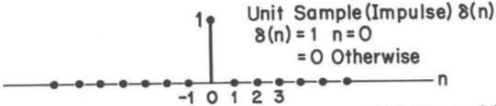
\includegraphics[width=\linewidth]{img/img002}
	\end{center}
\end{frame}

\begin{frame}
	\frametitle{Unit Sample Waktu Kontinyu}
	\begin{multicols}{2}
		\begin{center}
			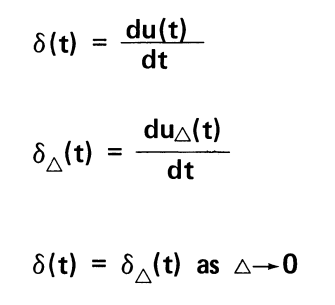
\includegraphics[width=0.7\linewidth]{img/img004}
		\end{center}
	\columnbreak
		\begin{center}
			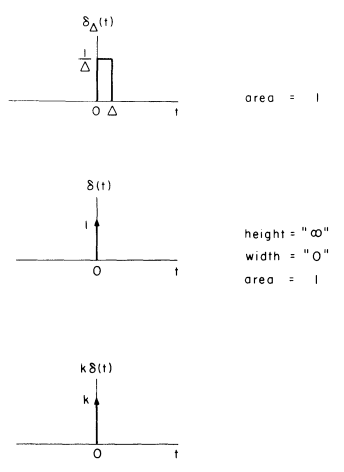
\includegraphics[width=0.9\linewidth]{img/img005}
		\end{center}
	\end{multicols}
\end{frame}

\begin{frame}
	\frametitle{Unit Step Sequence}
	\begin{itemize}
		\item Basic sequence yang kedua adalah \textbf{unit step sequence} yang diilustrasikan pada slide berikutnya.
		\item Unit step sequence dinotasikan dengan $ u[n] $.
		\item $ u(n) $ bernilai 1 (\textbf{unity}) saat $ n \geq 0 $ dan bernilai 0 saat $ n < 0 $.
		\item Berdasarkan definisi di atas, unit step sequence lebih mudah daripada unit step waktu kontinyu.
		\item Masih ingat dengan unit step waktu kontinyu?
	\end{itemize}
\end{frame}

\begin{frame}
	\frametitle{Unit Step Sequence}
	\begin{center}
		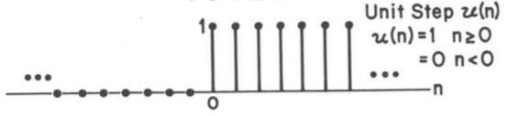
\includegraphics[width=\linewidth]{img/img003}
	\end{center}
\end{frame}

\begin{frame}
	\frametitle{Unit Step Waktu Kontinyu}
	\begin{center}
		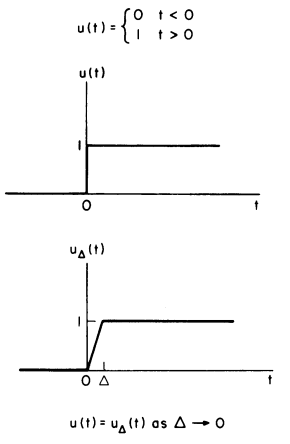
\includegraphics[height=0.9\textheight]{img/img006}
	\end{center}
\end{frame}

\begin{frame}
	\begin{itemize}
		\item<1-> Dalam domain waktu diskrit, terdapat keterkaitan/hubungan sederhana antara unit sample sequence dengan unit step sequence.
		\item<2-> Ada yang tahu?
		\item<3-> Unit sample sequence dapat diperoleh dari unit step sequence dengan cara membuat persamaan beda.
		\item<3-> Unit sample sequence $ \delta (n) $ sama dengan unit step, $ u(n) $, dikurangi dengan unit step yang di-delay sebanyak 1 sample.
		\item<4-> Perhatikan ilustrasinya di slide selanjutnya.
	\end{itemize}
\end{frame}

\begin{frame}
	\frametitle{Unit-sample sequence dalam bentuk unit-step sequence}
	\begin{center}
		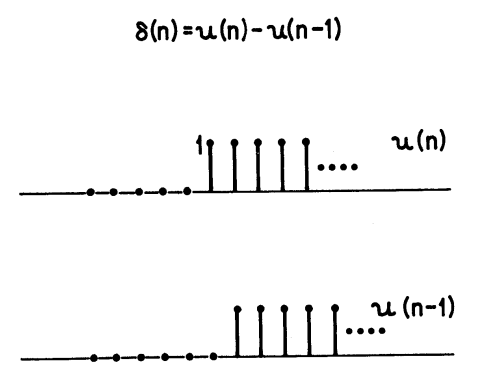
\includegraphics[height=0.8\textheight]{img/img007}
	\end{center}
\end{frame}

\begin{frame}
	\begin{itemize}
		\item Begitu juga untuk unit step sequence.
		\item Unit step sequence dapat diperoleh dari running sum dari unit sample sequence.
		\item Perhatikan ilustrasi pada slide selanjutnya.
	\end{itemize}
\end{frame}

\begin{frame}
	\frametitle{Unit-step sequence dalam bentuk unit-sample sequence}
	\begin{center}
		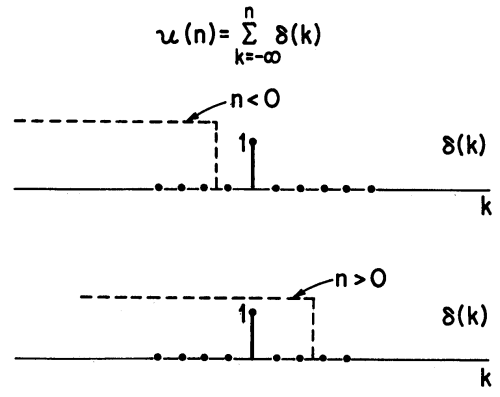
\includegraphics[height=0.8\textheight]{img/img008}
	\end{center}
\end{frame}

\begin{frame}
	\frametitle{Real exponential sequence}
	\begin{itemize}
		\item Basic sequence yang ketiga adalah \textbf{real exponential sequence}, $ x(n) = (\alpha)^n $.
		\item Jika $ 0 < \alpha < 1 $ maka eksponensial turun.
		\item Jika $ \alpha > 1 $ maka eksponensial naik.
	\end{itemize}
	\begin{center}
		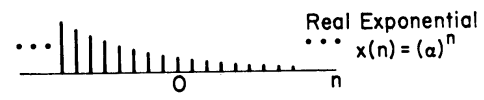
\includegraphics[width=0.8\linewidth]{img/img009}
	\end{center}
\end{frame}

\begin{frame}
	\frametitle{Sinusoidal sequence}
	\begin{itemize}
		\item Basic sequence yang keempat adalah \textbf{sinusoidal sequence}, $ x(n) = A\cos(\omega_0 n + \phi) $.
		\item $ A $ adalah amplitude, $ \omega_0 $ adalah frekuensi, dan $ \phi $ adalah sudut fasa.
		\item Contoh sinusoidal sequence di bawah ini adalah periodik.
		\item \textbf{Apakah sinusoidal seqence selalu periodik?} (\textit{Beri komen 1 untuk ya, dan 0 untuk tidak}).
	\end{itemize}
	\begin{center}
		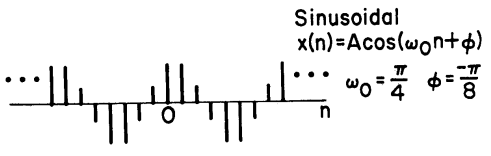
\includegraphics[width=0.8\linewidth]{img/img010}
	\end{center}
\end{frame}

\begin{frame}
	\frametitle{Sinusoidal sequence}
	\begin{center}
		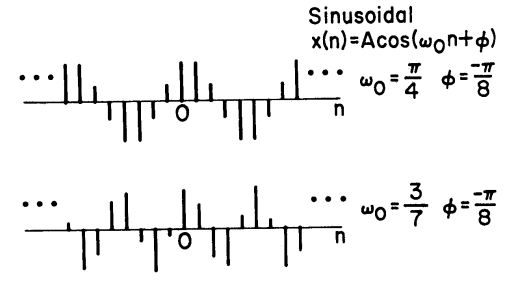
\includegraphics[width=0.8\linewidth]{img/img011}
	\end{center}
	\begin{itemize}
		\item Apakah sinusoidal sequence dengan $ \omega_0 = \frac{3}{7} $ adalah periodik? Ada yang bisa jelaskan?
	\end{itemize}
\end{frame}

\begin{frame}
	\frametitle{Sinusoidal sequence}
		\begin{itemize}
		\item Selain itu, hal yang perlu diperhatikan adalah sinusoidal sequence akan berbeda hanya jika $0 < \omega_0 < 2\pi $ atau $ -\pi < \omega_0 < \pi $.
		\item Karena jika kita mengganti $ \omega_0 $ dengan $ \omega_0 + 2\pi $, akan menghasilkan sequence yang sama.
	\end{itemize}
	\begin{center}
		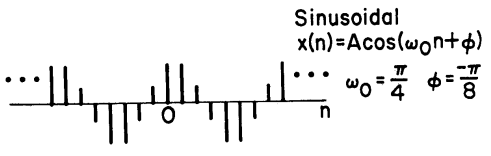
\includegraphics[width=0.8\linewidth]{img/img010}
	\end{center}
\end{frame}

\begin{frame}
	\frametitle{Merepresentasi sinyal dengan menggunakan basic sequence}
	\begin{itemize}
		\item Basic sequence dapat digunakan untuk merepresentasikan sinyal yang lebih luas.
		\item Sama seperti di domain waktu kontinyu, kita bisa menggunakan impulse, eksponensial kompleks, atau sionusoidal untuk merepresentasikan sinyal yang lebih luas.
		\item Perhatikan ilustrasi pada slide selanjutnya.
	\end{itemize}
\end{frame}

\begin{frame}
	\frametitle{Merepresentasi sinyal dengan menggunakan basic sequence}
	\begin{center}
		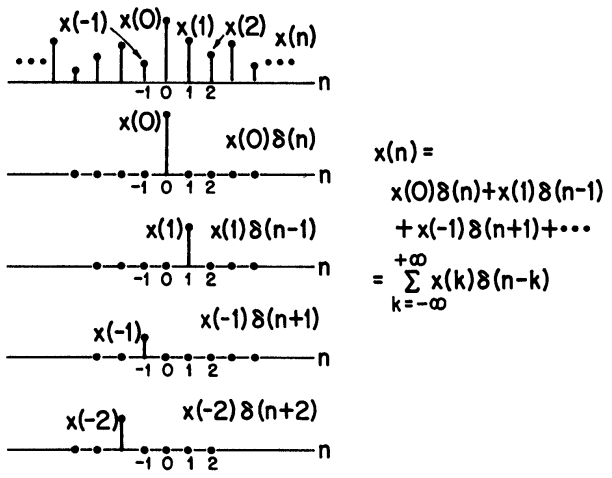
\includegraphics[width=0.8\linewidth]{img/img012}
	\end{center}
\end{frame}

\section{Sistem}

\begin{frame}
	\frametitle{General System}
	\begin{center}
		\includegraphics[width=0.5\linewidth]{img/img013}
	\end{center}
	\begin{itemize}
		\item input $ x(n) $, output $ y(n) $, dan sistem transformasi $ T[~] $.
	\end{itemize}
\end{frame}

\begin{frame}
	\frametitle{Special Class of System}
	\begin{itemize}
		\item Dalam mengkarakterisasi sistem, perlu memperhatikan kelas dari sistem tersebut.
		\item Kelas khusus dari sistem: 
		\begin{enumerate}
			\item \textbf{Linear}
			\item \textbf{Shift-invariant}
		\end{enumerate}
		\item Keduanya adalah independent, namun jika digabungan menghasilkan kelas khusus yaitu Linear \& Shift-invariant (\textbf{LSI}).
		\item Mirip dengan linear \& time-invariant di domain waktu kontinyu.
	\end{itemize}
\end{frame}

\begin{frame}
	\frametitle{Linearity}
	\begin{itemize}
		\item Jika diberikan input $ x_1(n) $ maka sistem akan memberikan output $ y_1(n) $. Dan jika diberikan input $ x_2(n) $ maka sistem yang sama akan memberikan output $ y_2(n) $.
		\begin{align*}
			x_1(n) &\rightarrow y_1(n) \\
			x_2(n) &\rightarrow y_2(n)
		\end{align*}
		\item Sistem tersebut dikatakan linier jika memiliki sifat linear combination antara input dan output dari sistem tersebut.
		\[ ax_1(n) + bx_2(n) \rightarrow ay_1(n) + by_2(n)\]
		\item Dengan kata lain, persamaan umumnya:
		\[ \sum a_k x_k(n) \rightarrow \sum a_k y_k(n) \]
	\end{itemize}
\end{frame}

\begin{frame}
	\frametitle{Shift-Invariance}
	\begin{itemize}
		\item Jika diberikan input $ x(n) $ maka sistem akan memberikan output $ y(n) $. Dan jika diberikan input $ x(n-n_0) $ maka sistem yang sama akan memberikan output $ y(n-n_0) $.
		\item Misalnya unit sample response:
		\begin{align*}
			\delta(n) &\rightarrow h(n) \\
			\delta(n-k) &\rightarrow h(n-k)
		\end{align*}
	\end{itemize}
\end{frame}

\begin{frame}
	\frametitle{Linear Shift-Invariance}
	\begin{itemize}
		\item Misalkan ada input \[ x(n) = \sum_{k = -\infty}^{k = +\infty} x(k)\delta(n-k) \]
		maka akan menghasilkan \[ y(n) = \sum_{k = -\infty}^{k = +\infty} x(k)h(n-k) \]
		\item Dari sini bisa kita pahami bahwa untuk mengkarakterisasi suatu sistem, kita bisa melihat unit sample response-nya.
		\item Disebut juga \textbf{convolution sum} (analogi dari convolution  integral di domain waktu kontinyu)
	\end{itemize}
\end{frame}

\begin{frame}
	\frametitle{Linear Shift-Invariance}
	\begin{itemize}
		\item<1-> Tapi ada karakteristik lainnya yang penting.
		\item<2-> Substitusi $ n - k $ dengan $ r $
		\[ n-k = r \rightarrow k = n-r\]
		\[ y(n) = \sum_{k = -\infty}^{k = +\infty} x(k)h(n-k) \rightarrow y(n) = \sum_r x(n-r)h(r) \]
		\item<3-> Coba perhatikan apa yang dapat kita simpulkan?
		\item<4-> Sistem tidak peduli mana yang kita sebut dengan input terhadap sistem dan mana yang kita sebut dengan unit sample response dari sistem.
	\end{itemize}
\end{frame}

\begin{frame}
	\frametitle{Convolution}
	\begin{itemize}
		\item Dengan kata lain, convolution bersifat komutatif:
		\begin{align*}
			y(n) &= x(n) * h(n) \\
			&= h(n) * x(n)
		\end{align*}
		\begin{center}
			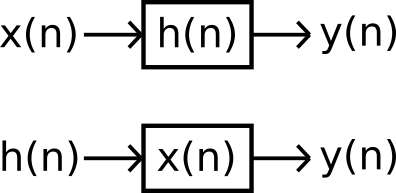
\includegraphics[width=0.3\linewidth]{img/img014}
		\end{center}
		\item Implikasinya adalah dalam cascade system:
		\begin{center}
			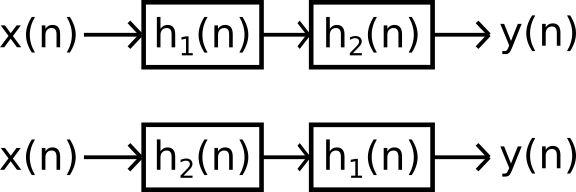
\includegraphics[width=0.4\linewidth]{img/img015}
		\end{center}
	\end{itemize}
\end{frame}

\begin{frame}
	\frametitle{Convolution}
	\begin{center}
		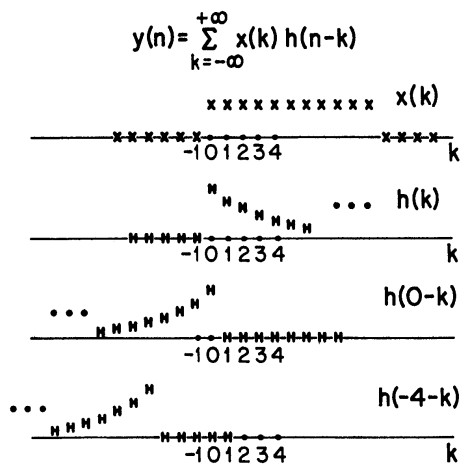
\includegraphics[height=0.8\textheight]{img/img016}
	\end{center}
\end{frame}

\begin{frame}
	\begin{center}
		
\includegraphics[width=\linewidth]{../../img/thank_you}
	\end{center}
	
\end{frame}

\begin{frame}
	\begin{center}
		
\includegraphics[width=\linewidth]{../../img/any_questions.png}
	\end{center}
\end{frame}

\section{Referensi}

\begin{frame}
	\frametitle{Referensi}
	\begin{itemize}
		\item Oppenheim, A. V., \& Schafer, R. W. (2014). Discrete-Time Signal Processing 3rd Edition. Boston: Pearson.
	\end{itemize}
\end{frame}

\end{document}